\chapter{Latches, Flip-Flops and Synchronous Sequential Circuits}\label{ch:latches}

\begin{objectives}
After studying this chapter you will be able to:
\begin{itemize}
  \item explain why a digital system needs memory and describe the general structure of a sequential circuit;
  \item distinguish synchronous from asynchronous circuits, and level-triggered latches from edge-triggered flip-flops;
  \item describe the operation of the SR, $\overline{S}\overline{R}$, gated SR and D latches, and of the D, JK and T flip-flops, using characteristic tables and equations;
  \item write VHDL for latches and flip-flops, with synchronous and asynchronous reset;
  \item analyse a clocked sequential circuit by deriving its state table and state diagram;
  \item distinguish the Mealy and Moore models; and
  \item design a synchronous sequential circuit with D, JK and T flip-flops using excitation tables.
\end{itemize}
\end{objectives}

\section{Why Sequential Circuits?}
The combinational circuits of Chapters~2--5 have one limitation: their output depends \emph{only} on the present input, and they have no memory of the past. Many real systems need such a memory:
\begin{itemize}
  \item a \textbf{vending machine} must know how much money \emph{has been} inserted;
  \item a \textbf{combination lock} must know whether the \emph{previous} digits were correct;
  \item a \textbf{counter} must know its \emph{present} value to compute the next.
\end{itemize}
The information that must be remembered is called the \term{state} of the system, and circuits that store it are built from \emph{memory elements}: latches and flip-flops.

\section{Structure of a Sequential Circuit}
A \term{sequential circuit} (\cref{fig:seq-block}) consists of a combinational circuit and memory elements connected in a loop. The memory elements hold the \emph{present state}; the combinational logic computes the \emph{next state} and the \emph{outputs} from the inputs and the present state; and the next state is stored in the memory elements at the next clock pulse. The feedback loop through the memory is what distinguishes a sequential from a combinational circuit.

\figside{472.2pt}{lect_6_sequential_circuit_block}{Block diagram of a sequential circuit: combinational logic, memory elements and the state feedback.}{fig:seq-block}

Sequential circuits are of two kinds.
\begin{itemize}
  \item In a \term{synchronous} sequential circuit state changes happen only at discrete instants, determined by a periodic signal called the \term{clock}. The memory elements are \emph{flip-flops}. Synchronous design is the dominant style because it is easier to design and verify and avoids many timing problems.
  \item In an \term{asynchronous} sequential circuit the state may change whenever an input changes. The memory elements are often simple \emph{latches}. Asynchronous circuits are faster but difficult to design reliably, and are outside the scope of this book.
\end{itemize}

\section{Latches}\label{sec:latches}
A \term{latch} is the simplest memory element: a circuit with two stable states, a \emph{bistable} circuit, that can store one bit as long as power is applied.

\subsection{The SR latch}
The \term{SR latch} (\cref{fig:sr-nor}) consists of two cross-coupled NOR gates; the inputs are \emph{Set} ($S$) and \emph{Reset} ($R$). Its behaviour (\cref{tab:sr-nor}) is:
\begin{itemize}
  \item $S=R=0$: no change; the latch remembers its state;
  \item $S=1,R=0$: \emph{set}: $Q=1$;
  \item $S=0,R=1$: \emph{reset}: $Q=0$;
  \item $S=R=1$: \emph{forbidden}: both outputs go to 0, violating $Q'=\overline{Q}$, and when both inputs return to 0 simultaneously the final state is unpredictable. This input combination must be avoided.
\end{itemize}
The memory comes from the feedback: when $S=R=0$ each gate acts as an inverter, and the two inverters in a loop hold whatever state they have.

\begin{table}[htbp]
\centering
\caption{SR latch with NOR gates.}
\label{tab:sr-nor}
\begin{tabular}{cc|cc|l}
\toprule
$S$&$R$&$Q(t+1)$&$Q'(t+1)$&State\\ \midrule
0&0&$Q$&$Q'$&no change\\0&1&0&1&reset\\1&0&1&0&set\\1&1&0&0&invalid\\ \bottomrule
\end{tabular}
\end{table}

\subsection{The $\overline{S}\overline{R}$ latch}
With NAND gates the same circuit has \emph{active-low} inputs, $\overline{S}$ and $\overline{R}$ (\cref{fig:sr-nand}, \cref{tab:sr-nand}): $(\overline{S},\overline{R})=(1,1)$ holds the state, $(0,1)$ sets, $(1,0)$ resets, and $(0,0)$ is invalid (both outputs 1).

\begin{table}[htbp]
\centering
\caption{$\overline{S}\overline{R}$ latch with NAND gates.}
\label{tab:sr-nand}
\begin{tabular}{cc|cc|l}
\toprule
$\overline{S}$&$\overline{R}$&$Q(t+1)$&$Q'(t+1)$&State\\ \midrule
0&0&1&1&invalid\\0&1&1&0&set\\1&0&0&1&reset\\1&1&$Q$&$Q'$&no change\\ \bottomrule
\end{tabular}
\end{table}

\begin{figure}[htbp]
\centering
\begin{subfigure}[b]{129.4pt}\centering
  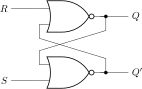
\includegraphics[width=127.4pt]{lect_6_sr_latch_nor}\caption{NOR SR latch}\label{fig:sr-nor}
\end{subfigure}
\hfill
\begin{subfigure}[b]{129.4pt}\centering
  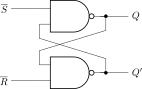
\includegraphics[width=127.4pt]{lect_6_sr_latch_nand}\caption{NAND $\overline{S}\overline{R}$ latch}\label{fig:sr-nand}
\end{subfigure}
\caption{Basic latches built from cross-coupled gates.}
\end{figure}

\subsection{Gated SR latch and D latch}
Adding two gates and a control input $C$ makes the latch respond to $S$ and $R$ only while $C=1$ (\cref{fig:gated}a): when $C=0$ the latch holds its state. This is the \term{gated SR latch}. To remove the forbidden input combination, an inverter ensures that $S$ and $R$ are never 1 together: connect $S=D$ and $R=D'$. The result is the \term{D latch} (\cref{fig:gated}b, \cref{tab:dlatch}): while $C=1$, $Q$ follows $D$ (the latch is \emph{transparent}); when $C=0$ the latch holds the last value of $D$. Its equation is $Q(t+1)=D$ when $C=1$.

\begin{table}[htbp]
\centering
\caption{D latch.}
\label{tab:dlatch}
\begin{tabular}{cc|l}
\toprule $C$&$D$&$Q(t+1)$\\ \midrule 0&X&no change\\1&0&0 (reset)\\1&1&1 (set)\\ \bottomrule \end{tabular}
\end{table}

\begin{figure}[htbp]
\centering
\begin{subfigure}[b]{207.4pt}\centering
  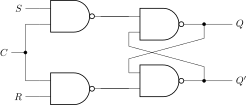
\includegraphics[width=205.4pt]{lect_6_gated_sr_latch}\caption{gated SR latch}
\end{subfigure}
\\[6pt]
\begin{subfigure}[b]{250.5pt}\centering
  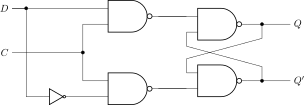
\includegraphics[width=248.5pt]{lect_6_d_latch}\caption{D latch}
\end{subfigure}
\caption{Gated latches.}\label{fig:gated}
\end{figure}

\figw{292.1pt}{lect_6_latch_symbols}{Graphical symbols of the SR, $\overline{S}\overline{R}$ and D latches.}{fig:latch-symbols}

\vhdlfile{listings/ch06_d_latch.vhd}{A D latch. The process is sensitive to both \code{D} and \code{C}; since no value is assigned when \code{C} is 0, the synthesis tool infers a latch.}{lst:dlatch}

\Cref{lst:dlatch} shows how a latch is described: the process has no \code{else} branch, so \code{Q} keeps its value when \code{C = '0'}, which means memory. Unintentional latches caused by incomplete \code{if} statements are a common mistake in combinational VHDL descriptions.

\section{Flip-Flops}\label{sec:flipflops}
A latch is \term{level-triggered}: its output may change at any time while the control input is active. In a circuit in which the latch output feeds back into its own input through combinational logic this causes uncontrolled multiple transitions during one clock pulse. A \term{flip-flop} is \term{edge-triggered}: it samples its inputs and changes state only at one \emph{edge} of the clock (\cref{fig:trigger}), so that all state changes in a synchronous system happen at the same moment. In a \emph{positive-edge} flip-flop the transition is on the rising edge (0 $\to$ 1), in a \emph{negative-edge} flip-flop on the falling edge (1 $\to$ 0).

\figw{191.7pt}{lect_6_trigger_types}{Level triggering, positive-edge triggering and negative-edge triggering.}{fig:trigger}

\subsection{The D flip-flop}
The D flip-flop is the most common flip-flop. At the active clock edge it captures the value of $D$ and stores it in $Q$. One way to build it is the \emph{master--slave} configuration of \cref{fig:ms}: two D latches in series with opposite clock polarity. While CLK is 1 the master latch is transparent and follows $D$ while the slave is closed and holds the old value. When CLK falls to 0 the master closes, capturing $D$, and the slave opens and passes the captured value to $Q$. $Q$ therefore changes only when the clock falls: a negative-edge D flip-flop. The characteristic equation is $Q(t+1)=D$.

\begin{figure}[htbp]
\centering
\begin{subfigure}[b]{208.9pt}\centering
  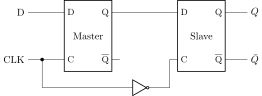
\includegraphics[width=206.9pt]{lect_6_master_slave_d_flip_flop}\caption{master--slave construction}
\end{subfigure}
\hfill
\begin{subfigure}[b]{145.3pt}\centering
  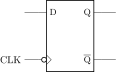
\includegraphics[width=143.3pt]{lect_6_d_flip_flop_neg_edge}\caption{symbols}
\end{subfigure}
\caption{Edge-triggered D flip-flop.}\label{fig:ms}
\end{figure}

\subsection{The JK flip-flop}
The \term{JK flip-flop} refines the SR flip-flop by giving meaning to the forbidden input. $J$ sets, $K$ resets, and when $J=K=1$ the flip-flop \emph{toggles}: $Q$ becomes $Q'$. Its characteristic equation is
\[
 Q(t+1) = JQ' + K'Q .
\]
A JK flip-flop can be built from a D flip-flop with the input equation $D=JQ'+K'Q$ (\cref{fig:jk}).

\subsection{The T flip-flop}
The \term{T flip-flop} has a single input $T$: if $T=0$ it holds its state and if $T=1$ it toggles, $Q(t+1)=T\xor Q$. It is useful for counters. It is obtained from a JK flip-flop by tying $J=K=T$, or from a D flip-flop with an XOR gate, $D=T\xor Q$ (\cref{fig:tff}).

\begin{figure}[htbp]
\centering
\begin{subfigure}[b]{304.6pt}\centering
  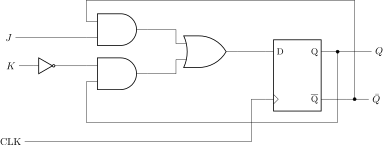
\includegraphics[width=302.6pt]{lect_6_jk_flip_flop_from_d}\caption{JK from a D flip-flop}
\end{subfigure}
\\[6pt]
\begin{subfigure}[b]{145.3pt}\centering
  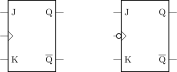
\includegraphics[width=143.3pt]{lect_6_jk_flip_flop_symbol}\caption{JK symbol}
\end{subfigure}
\caption{JK flip-flop.}\label{fig:jk}
\end{figure}

\begin{figure}[htbp]
\centering
\begin{subfigure}[b]{145.3pt}\centering
  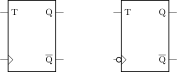
\includegraphics[width=143.3pt]{lect_6_t_flip_flop_symbol}\caption{symbol}
\end{subfigure}
\hfill
\begin{subfigure}[b]{124.0pt}\centering
  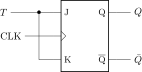
\includegraphics[width=122.0pt]{lect_6_t_flip_flop_from_jk}\caption{from JK}
\end{subfigure}
\\[6pt]
\begin{subfigure}[b]{180.6pt}\centering
  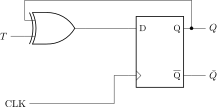
\includegraphics[width=178.6pt]{lect_6_t_flip_flop_from_d}\caption{from D and XOR}
\end{subfigure}
\caption{T flip-flop.}\label{fig:tff}
\end{figure}

\subsection{Characteristic tables}
The behaviour of each flip-flop is summarised by its \term{characteristic table}, which gives the next state $Q(t+1)$ as a function of the inputs and the present state $Q(t)$, and by the equivalent \term{characteristic equation} (\cref{tab:char}). The SR equation $Q(t+1)=S+R'Q$ holds under the restriction $SR=0$.

\begin{table}[htbp]
\centering
\caption{Characteristic tables and equations of the flip-flops.}
\label{tab:char}
\begin{tabular}{@{}cccc@{}}
\toprule
\textbf{SR} & \textbf{D} & \textbf{JK} & \textbf{T}\\ \midrule
$Q(t{+}1)=S+R'Q$ & $Q(t{+}1)=D$ & $Q(t{+}1)=JQ'+K'Q$ & $Q(t{+}1)=T\xor Q$\\[4pt]
\begin{tabular}{cc|c}$S$&$R$&$Q(t{+}1)$\\\hline0&0&$Q$\\0&1&0\\1&0&1\\1&1&?\end{tabular}&
\begin{tabular}{c|c}$D$&$Q(t{+}1)$\\\hline0&0\\1&1\end{tabular}&
\begin{tabular}{cc|c}$J$&$K$&$Q(t{+}1)$\\\hline0&0&$Q$\\0&1&0\\1&0&1\\1&1&$Q'$\end{tabular}&
\begin{tabular}{c|c}$T$&$Q(t{+}1)$\\\hline0&$Q$\\1&$Q'$\end{tabular}\\
\bottomrule
\end{tabular}
\end{table}

\subsection{VHDL descriptions}
In VHDL a flip-flop is described by a process that is sensitive to the clock and does something only at the active edge, detected with the function \code{rising_edge(CLK)} (or \code{falling_edge}). The assignments made in such a process are \emph{registered}: the synthesis tool creates flip-flops. \Cref{lst:dff,lst:jkff,lst:tff} show the D, JK and T flip-flops.

\vhdlfile{listings/ch06_d_ff.vhd}{A positive-edge-triggered D flip-flop.}{lst:dff}
\vhdlfile{listings/ch06_jk_ff.vhd}{A JK flip-flop. The internal signal \code{q_int} lets the value of \code{Q} be read back for the toggle operation.}{lst:jkff}
\vhdlfile{listings/ch06_t_ff.vhd}{A T flip-flop.}{lst:tff}

\subsection{Asynchronous and synchronous reset}
Flip-flops often have \emph{preset} (set $Q=1$) and \emph{clear} or \emph{reset} (set $Q=0$) inputs, shown with a bubble if active-low (\cref{fig:ffpr}). A reset can act in two ways.
\begin{itemize}
  \item An \term{asynchronous} reset overrides the clock and the data input: the output changes \emph{immediately} when the reset becomes active. In VHDL the reset is tested \emph{before} the clock-edge condition (\cref{lst:async}).
  \item A \term{synchronous} reset takes effect only at the active clock edge. In VHDL the reset is tested \emph{inside} the clock-edge condition (\cref{lst:sync}).
\end{itemize}
Asynchronous reset is convenient for initialising a system at power-up; synchronous reset keeps all state changes aligned with the clock. Releasing an asynchronous reset close to a clock edge can cause timing violations, so in practice the reset signal is itself synchronised to the clock.

\figw{242.0pt}{lect_6_d_ff_preset_reset}{D flip-flops with asynchronous preset and clear inputs.}{fig:ffpr}

\vhdlfile{listings/ch06_async_reset.vhd}{Process with asynchronous reset.}{lst:async}
\vhdlfile{listings/ch06_sync_reset.vhd}{Process with synchronous reset.}{lst:sync}

\section{Analysis of Clocked Sequential Circuits}\label{sec:seq-analysis}
\termx{Analysis}{analysis} derives the behaviour of a given sequential circuit, expressed as a \term{state table} or \term{state diagram}.
\begin{enumerate}
  \item From the logic diagram, write the \term{flip-flop input equations} (excitation equations) and the \term{output equations}.
  \item Substitute the input equations in the characteristic equation of each flip-flop to obtain the \emph{next-state equations}: $Q(t+1)=D$ for a D flip-flop, $Q(t+1)=JQ'+K'Q$ for JK, $Q(t+1)=T\xor Q$ for T.
  \item Construct the \term{state table}, which lists the next state and the output for every combination of present state and input.
  \item Draw the \term{state diagram}: a circle for each state and an arrow for each transition, labelled \texttt{input/output}.
\end{enumerate}

\begin{example}{Analysis with D flip-flops}{seq-d}
The circuit of \cref{fig:seq-d} has two D flip-flops $A$ and $B$, an input $x$ and an output $y$.

\textbf{Equations.} $D_A=Ax+Bx$, $D_B=A'x$, $y=A+Bx'$. Since $A(t+1)=D_A$ and $B(t+1)=D_B$, the next-state equations are $A(t+1)=Ax+Bx$ and $B(t+1)=A'x$.

\textbf{State table.} Evaluating these equations for the eight combinations of $AB$ and $x$ gives \cref{tab:seq-d}; the corresponding state diagram is \cref{fig:seq-d-state}.
\end{example}

\begin{table}[htbp]
\centering
\caption{State table of \cref{ex:seq-d}.}
\label{tab:seq-d}
\begin{tabular}{cc|c|cc|c}
\toprule
\multicolumn{2}{c|}{Present state} & Input & \multicolumn{2}{c|}{Next state} & Output\\
$A$&$B$&$x$&$A$&$B$&$y$\\ \midrule
0&0&0&0&0&0\\0&0&1&0&1&0\\0&1&0&0&0&1\\0&1&1&1&1&0\\
1&0&0&0&0&1\\1&0&1&1&0&0\\1&1&0&0&0&1\\1&1&1&1&0&0\\ \bottomrule
\end{tabular}
\end{table}

\begin{figure}[htbp]
\centering
\begin{subfigure}[b]{402.8pt}\centering
  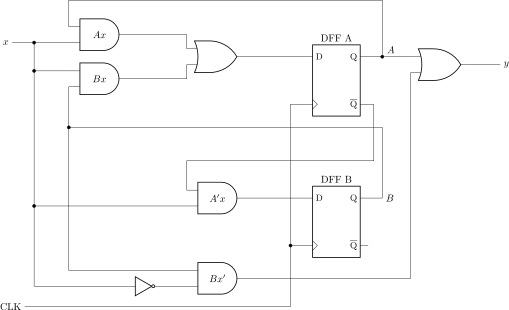
\includegraphics[width=400.8pt]{lect_6_sequential_analysis_example}\caption{circuit}\label{fig:seq-d}
\end{subfigure}
\\[6pt]
\begin{subfigure}[b]{131.8pt}\centering
  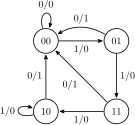
\includegraphics[width=129.8pt]{lect_6_d_state_diagram}\caption{state diagram}\label{fig:seq-d-state}
\end{subfigure}
\caption{The circuit analysed in \cref{ex:seq-d}.}
\end{figure}

\begin{example}{Analysis with JK flip-flops}{seq-jk}
In \cref{fig:seq-jk} the inputs are $J_A=B$, $K_A=Bx'$, $J_B=x'$, $K_B=A'x+Ax'=A\xor x$. With $Q(t+1)=JQ'+K'Q$,
\[
 A(t+1)=BA'+(Bx')'A,\qquad B(t+1)=x'B'+(A\xor x)'B .
\]
\Cref{tab:seq-jk} lists the flip-flop inputs for each row and the resulting next state, which gives the state diagram of \cref{fig:seq-jk-state}. (Row $AB=01$, $x=0$: $J_A=1,K_A=1$ toggles $A$ from 0 to 1, and $J_B=1,K_B=0$ sets $B$, so the next state is 11.)
\end{example}

\begin{table}[htbp]
\centering
\caption{State table of \cref{ex:seq-jk}.}
\label{tab:seq-jk}
\begin{tabular}{cc|c|cccc|cc}
\toprule
\multicolumn{2}{c|}{Present state} & Input & \multicolumn{4}{c|}{Flip-flop inputs} & \multicolumn{2}{c}{Next state}\\
$A$&$B$&$x$&$J_A$&$K_A$&$J_B$&$K_B$&$A$&$B$\\ \midrule
0&0&0&0&0&1&0&0&1\\0&0&1&0&0&0&1&0&0\\0&1&0&1&1&1&0&1&1\\0&1&1&1&0&0&1&1&0\\
1&0&0&0&0&1&1&1&1\\1&0&1&0&0&0&0&1&0\\1&1&0&1&1&1&1&0&0\\1&1&1&1&0&0&0&1&1\\ \bottomrule
\end{tabular}
\end{table}

\begin{figure}[htbp]
\centering
\begin{subfigure}[b]{295.1pt}\centering
  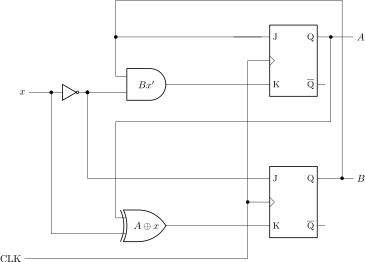
\includegraphics[width=293.1pt]{lect_6_jk_sequential_analysis}\caption{circuit}\label{fig:seq-jk}
\end{subfigure}
\\[6pt]
\begin{subfigure}[b]{137.8pt}\centering
  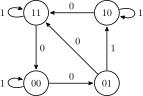
\includegraphics[width=135.8pt]{lect_6_jk_state_diagram}\caption{state diagram}\label{fig:seq-jk-state}
\end{subfigure}
\caption{The circuit analysed in \cref{ex:seq-jk}.}
\end{figure}

\begin{example}{Analysis with T flip-flops}{seq-t}
In \cref{fig:seq-t}: $T_A=Bx$, $T_B=x$ and $y=AB$. With $Q(t+1)=T\xor Q$, $A(t+1)=Bx\xor A$ and $B(t+1)=x\xor B$. The state table is \cref{tab:seq-t}. Because $y=AB$ depends on the state only, the machine is a \emph{Moore} machine and its diagram (\cref{fig:seq-t-state}) writes the output inside each state, \texttt{state/output}, and labels the arrows with the input.
\end{example}

\begin{table}[htbp]
\centering
\caption{State table of \cref{ex:seq-t}.}
\label{tab:seq-t}
\begin{tabular}{cc|c|cc|c}
\toprule
\multicolumn{2}{c|}{Present state} & Input & \multicolumn{2}{c|}{Next state} & Output\\
$A$&$B$&$x$&$A$&$B$&$y$\\ \midrule
0&0&0&0&0&0\\0&0&1&0&1&0\\0&1&0&0&1&0\\0&1&1&1&0&0\\
1&0&0&1&0&0\\1&0&1&1&1&0\\1&1&0&1&1&1\\1&1&1&0&0&1\\ \bottomrule
\end{tabular}
\end{table}

\begin{figure}[htbp]
\centering
\begin{subfigure}[b]{377.3pt}\centering
  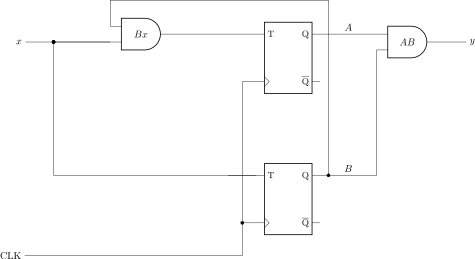
\includegraphics[width=375.3pt]{lect_6_t_sequential_analysis}\caption{circuit}\label{fig:seq-t}
\end{subfigure}
\\[6pt]
\begin{subfigure}[b]{148.8pt}\centering
  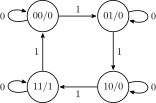
\includegraphics[width=146.8pt]{lect_6_t_state_diagram}\caption{state diagram}\label{fig:seq-t-state}
\end{subfigure}
\caption{The circuit analysed in \cref{ex:seq-t}.}
\end{figure}

\section{Mealy and Moore Models}\label{sec:mealymoore}
Synchronous sequential circuits are classified by how their outputs are generated.
\begin{itemize}
  \item In the \term{Mealy model}~\cite{mealy1955} the outputs depend on the \emph{present state and the present inputs}. In a state diagram the output is written on each transition, \texttt{input/output}. Because the output depends directly on the inputs, it can change between clock edges whenever the input changes, and may show momentary false values (glitches).
  \item In the \term{Moore model}~\cite{moore1956} the outputs depend \emph{only on the present state}. In a state diagram the output is written inside each state circle. Moore outputs change only when the state changes, which is just after a clock edge, so they are synchronous and glitch-free.
\end{itemize}
The two models are compared in detail, with timing diagrams, in \cref{sec:moore-mealy}.

\section{Design of Sequential Circuits}\label{sec:seq-design}
\termx{Design}{design} is the reverse of analysis: from a specification to a logic diagram.
\begin{enumerate}
  \item Derive a \textbf{state diagram} from the word description.
  \item Perform \textbf{state reduction}: remove states that are equivalent.
  \item Perform \textbf{state assignment}: assign a unique binary code to each state. A machine with $N$ states needs at least $\lceil\log_2N\rceil$ flip-flops.
  \item Write the binary-coded \textbf{state table}.
  \item Choose the \textbf{type of flip-flop}.
  \item Derive the simplified \textbf{flip-flop input equations} and \textbf{output equations} with K-maps (unused states give don't-cares).
  \item Draw the \textbf{logic diagram} (or write the VHDL) and verify it.
\end{enumerate}

\subsection{Example: a sequence detector}
\begin{example}{101 sequence detector}{seqdet}
Design a circuit with input $x$ and output $y$ that produces $y=1$ whenever the input sequence $101$ has just been received. Overlapping sequences count ($10101$ contains two).

\textbf{State diagram.} Three states are needed to remember how much of the pattern has been seen: $S_0$, the initial state (no useful input yet, or the last input was 0 without a preceding 1); $S_1$, the last input was 1; $S_2$, the last two inputs were 10. In $S_2$ a 1 completes the sequence: the output is 1 and, since the last input was 1, the next state is $S_1$. The output depends on the input, so this is a Mealy machine (\cref{fig:seqdet-state}).

\textbf{State assignment.} $S_0=00$, $S_1=01$, $S_2=10$; two flip-flops $A$ and $B$. The state $11$ is unused.

\textbf{State table} (\cref{tab:seqdet}).
\end{example}

\begin{table}[htbp]
\centering
\caption{State table of the 101 detector, $S_0=00$, $S_1=01$, $S_2=10$.}
\label{tab:seqdet}
\begin{tabular}{cc|c|cc|c}
\toprule
\multicolumn{2}{c|}{Present state} & Input & \multicolumn{2}{c|}{Next state} & Output\\
$A$&$B$&$x$&$A$&$B$&$y$\\ \midrule
0&0&0&0&0&0\\0&0&1&0&1&0\\0&1&0&1&0&0\\0&1&1&0&1&0\\
1&0&0&0&0&0\\1&0&1&0&1&1\\ \bottomrule
\end{tabular}
\end{table}

\figw{204.9pt}{lect_6_sequence_detector_state}{State diagram of the 101 sequence detector (Mealy).}{fig:seqdet-state}

\paragraph{Implementation with D flip-flops.} For D flip-flops the input equation is the next-state value. From K-maps of \cref{tab:seqdet} (with the unused state 11 as don't-care):
\[
 D_A = Bx',\qquad D_B = x,\qquad y = Ax .
\]
The circuit is shown in \cref{fig:seqdet-circuit}.

\figw{391.2pt}{lect_6_sequence_detector_circuit}{Logic diagram of the 101 detector with D flip-flops.}{fig:seqdet-circuit}

\paragraph{Excitation tables.} For JK and T flip-flops we need the \term{excitation table}, the inverse of the characteristic table: it states which flip-flop inputs produce a required transition $Q(t)\to Q(t+1)$ (\cref{tab:excit}). The X entries are don't-cares and are what make JK designs sometimes simpler than D designs.

\begin{table}[htbp]
\centering
\caption{Excitation tables of the JK and T flip-flops.}
\label{tab:excit}
\begin{tabular}{cc|cc}
\toprule \multicolumn{4}{c}{JK}\\ $Q(t)$&$Q(t{+}1)$&$J$&$K$\\ \midrule
0&0&0&X\\0&1&1&X\\1&0&X&1\\1&1&X&0\\ \bottomrule
\end{tabular}\qquad\qquad
\begin{tabular}{cc|c}
\toprule \multicolumn{3}{c}{T}\\ $Q(t)$&$Q(t{+}1)$&$T$\\ \midrule
0&0&0\\0&1&1\\1&0&1\\1&1&0\\ \bottomrule
\end{tabular}
\end{table}

\paragraph{Implementation with JK flip-flops.} We extend the state table with the required $J$ and $K$ inputs of each flip-flop (\cref{tab:seqdet-jk}). For flip-flop $A$: transition $0\to0$ needs $J_A=0$; $0\to1$ (row $AB=01$, $x=0$) needs $J_A=1$; $1\to0$ (both rows with $AB=10$) needs $K_A=1$. For flip-flop $B$: $0\to1$ occurs when $x=1$ in states 00 and 10; $1\to0$ in state 01 when $x=0$; $1\to1$ in state 01 when $x=1$. The K-maps (the unused state 11 and all entries X are don't-cares) give
\[
 J_A = Bx',\qquad K_A = 1,\qquad J_B = x,\qquad K_B = x',\qquad y = Ax .
\]
Note that $K_A$ is the constant 1: in state $10$ the flip-flop $A$ must always return to 0, whatever the input, and in all other states the value of $K_A$ is a don't-care. The flip-flop input logic of the JK design is thus one AND gate and one inverter (shared by $J_A$ and $K_B$), the same as for the D design; the advantage of JK flip-flops appears in larger machines, where the don't-cares often remove literals.

\begin{table}[htbp]
\centering
\caption{Excitation table for the 101 detector with JK flip-flops.}
\label{tab:seqdet-jk}
\begin{tabular}{cc|c|cc|cc|cc}
\toprule
\multicolumn{2}{c|}{PS} & Input & \multicolumn{2}{c|}{NS} & \multicolumn{2}{c|}{$A$ inputs} & \multicolumn{2}{c}{$B$ inputs}\\
$A$&$B$&$x$&$A$&$B$&$J_A$&$K_A$&$J_B$&$K_B$\\ \midrule
0&0&0&0&0&0&X&0&X\\0&0&1&0&1&0&X&1&X\\
0&1&0&1&0&1&X&X&1\\0&1&1&0&1&0&X&X&0\\
1&0&0&0&0&X&1&0&X\\1&0&1&0&1&X&1&1&X\\ \bottomrule
\end{tabular}
\end{table}

\paragraph{VHDL descriptions.} In VHDL a machine is best described with an \emph{enumerated type} for the states, e.g.\ \code{type state_type is (S0, S1, S2);}; the synthesis tool then chooses the state encoding (binary, one-hot, \dots). \Cref{lst:seqdet-fsm} describes the detector with two processes: a clocked process holding the state register and a combinational process computing the next state and the output. \Cref{lst:seqdet-struct} is the gate-level (structural) description that follows the D-flip-flop design.

\vhdlfile{listings/ch06_seq_detector_fsm.vhd}{The 101 detector as a state machine with an enumerated state type.}{lst:seqdet-fsm}
\vhdlfile{listings/ch06_seq_detector_struct.vhd}{The 101 detector as two D flip-flops and gates (structural description).}{lst:seqdet-struct}

\subsection{Example: a binary counter with T flip-flops}
\begin{example}{3-bit binary counter}{counter3}
Design a counter that cycles through $000,001,\dots,111$ and back to $000$, using T flip-flops. There are no inputs except the clock.

\textbf{Solution.} A T flip-flop must toggle ($T=1$) exactly when its bit changes between the present and next states. In the table, $A_0$ changes every clock; $A_1$ changes when $A_0=1$; $A_2$ changes when $A_1=A_0=1$ (\cref{tab:counter3}). Hence
\[
 T_{A_0}=1,\qquad T_{A_1}=A_0,\qquad T_{A_2}=A_1A_0 .
\]
The circuit (\cref{fig:counter3}) uses three flip-flops and one AND gate.
\end{example}

\begin{table}[htbp]
\centering
\caption{State table and T inputs of the 3-bit counter.}
\label{tab:counter3}
\begin{tabular}{ccc|ccc|ccc}
\toprule
\multicolumn{3}{c|}{Present state} & \multicolumn{3}{c|}{Next state} & \multicolumn{3}{c}{Flip-flop inputs}\\
$A_2$&$A_1$&$A_0$&$A_2$&$A_1$&$A_0$&$T_{A_2}$&$T_{A_1}$&$T_{A_0}$\\ \midrule
0&0&0&0&0&1&0&0&1\\0&0&1&0&1&0&0&1&1\\0&1&0&0&1&1&0&0&1\\0&1&1&1&0&0&1&1&1\\
1&0&0&1&0&1&0&0&1\\1&0&1&1&1&0&0&1&1\\1&1&0&1&1&1&0&0&1\\1&1&1&0&0&0&1&1&1\\ \bottomrule
\end{tabular}
\end{table}

\figw{314.0pt}{lect_6_t_3bit_counter}{A 3-bit binary counter with T flip-flops.}{fig:counter3}

\begin{chaptersummary}
\begin{itemize}
  \item A \textbf{sequential circuit} contains memory; its output depends on the inputs and the \textbf{state}. \textbf{Synchronous} circuits change state at clock edges, using flip-flops.
  \item \textbf{Latches} (SR, $\overline{S}\overline{R}$, gated SR, D) are level-triggered. \textbf{Flip-flops} (D, JK, T) are edge-triggered. Characteristic equations: $Q^+=D$; $Q^+=JQ'+K'Q$; $Q^+=T\xor Q$; $Q^+=S+R'Q$ ($SR=0$).
  \item \textbf{Asynchronous} reset overrides the clock; \textbf{synchronous} reset acts at the clock edge. In VHDL, \code{rising_edge(clk)} describes a flip-flop.
  \item \textbf{Analysis}: logic diagram $\to$ flip-flop input equations $\to$ next-state equations $\to$ state table $\to$ state diagram.
  \item \textbf{Mealy}: output depends on state and input. \textbf{Moore}: output depends on state only.
  \item \textbf{Design}: word problem $\to$ state diagram $\to$ (reduction) $\to$ state assignment $\to$ state table $\to$ excitation $\to$ flip-flop input equations $\to$ logic diagram. Use the \textbf{excitation tables} for JK and T flip-flops.
\end{itemize}
\end{chaptersummary}

\chapsec{Exercises}
\begin{exlist}
  \item \textbf{Next-state equations.} A sequential circuit has two D flip-flops $A$, $B$ and an input $x$, with $D_A=Ax+Bx$ and $D_B=A'x$. Write the next-state equations $A(t+1)$ and $B(t+1)$.
  \item \textbf{State diagram.} A circuit has one T flip-flop and an input $x$, with $T=A\xor x$. Draw the state diagram. Describe what the circuit does.
  \item \textbf{JK flip-flop behaviour.} A JK flip-flop has $J=K=1$ permanently. (a)~Describe how $Q$ changes on each clock pulse. (b)~Draw its state diagram. (c)~If the clock frequency is 1~MHz, what is the frequency of $Q$?
  \item \textbf{Mealy or Moore?} ``A sequence detector produces $y=1$ whenever the internal counter holds the value 101. The output remains 1 as long as the counter is in this state, regardless of the input during that clock cycle.'' Classify the machine and justify your answer.
  \item An NOR SR latch initially has $Q=0$. The inputs $(S,R)$ are applied in turn: $(0,0)$, $(1,0)$, $(0,0)$, $(0,1)$, $(0,0)$. Give $Q$ after each step.
  \item Explain why a D latch cannot be used directly in place of a D flip-flop in a counter in which $Q'$ is fed back to $D$. What happens while the latch is transparent?
  \item Show how to build (a)~a T flip-flop and (b)~a D flip-flop from a JK flip-flop.
  \item Derive the characteristic equation $Q(t+1)=S+R'Q$ of the SR flip-flop from its characteristic table, with a K-map in which the combination $S=R=1$ is a don't-care.
  \item \textbf{Analysis.} A circuit has two D flip-flops with $D_A=x\xor B$, $D_B=A$ and output $y=AB'$. Draw the state table and state diagram. Is it a Mealy or a Moore machine?
  \item \textbf{Design.} Design a Mealy sequence detector with input $x$ and output $y$ that detects the sequence $110$ (overlapping allowed) using two D flip-flops with the state assignment $S_0=00$, $S_1=01$, $S_2=10$. Give the state diagram, the state table, the equations, and the VHDL of the machine.
  \item Design a 3-bit binary counter with JK flip-flops.
  \item How many flip-flops are required to implement a state machine with (a)~5 states; (b)~9 states; (c)~a one-hot encoding of 9 states?
  \item Write VHDL for a D flip-flop with synchronous reset and an enable input \code{en}: the register loads \code{D} only when \code{en = '1'}.
  \item Write the VHDL of an 8-bit register with asynchronous active-low reset.
\end{exlist}

\chapsec{Further Reading}
The treatment of latches, flip-flops and the analysis and design of clocked sequential circuits follows Chapter~5 of Mano and Ciletti~\cite{mano2018}. Brown and Vranesic~\cite{brown2009} (Chapters~7 and~8) and Wakerly~\cite{wakerly2006} discuss timing parameters (setup, hold, propagation delay) in detail, which we have not covered. Mealy~\cite{mealy1955} and Moore~\cite{moore1956} introduced the two models. For VHDL coding style for registers and state machines, see Ashenden~\cite{ashenden2008}.
